\documentclass[french]{article}
\usepackage[T1]{fontenc}
\usepackage[utf8]{inputenc}
\usepackage[a4paper,top=3cm,bottom=2cm,left=1.5cm,right=1.5cm,headheight=60pt]{geometry}
\usepackage{babel} % gestion de la langue
\usepackage{float} % gestion des images
\usepackage{graphicx} % gestion des images
\usepackage{lipsum} % remplissage de texte
%\usepackage[parfill]{parskip} % pas d'indentation en début de paragraphe
\usepackage{libertine} % police d'écriture
\usepackage{multicol} % double colonne
\usepackage{fancyhdr} % gestion des en-têtes / pieds de page
\usepackage{fourier-orns}
\usepackage{pgfornament}
\usepackage{url}
\usepackage{amsmath}
% ============ HEADER / FOOTER =======================
\fancypagestyle{hdr-normal}{
  \renewcommand{\headrulewidth}{0pt}
  \renewcommand{\footrulewidth}{0pt}
    \fancyhead[L]{\bsc{Machine Learning} \\[-5pt] \vhrulefill{1pt} \hspace{70pt} \ \\ 2019-2020}%
    \fancyhead[C]{\bsc{Université de Rennes 1} \\[-5pt] \ \\ \bsc{UFR Sciences Économiques}}%
    \fancyhead[R]{\raisebox{-0.15\height}{\includegraphics[scale=0.1]{img/logo_r1n.png}}}
    \fancyfoot[L]{}
    \fancyfoot[C]{}
    \fancyfoot[R]{\bf\thepage}
}
\pagestyle{hdr-normal} % application en-têtes/pieds de page à l'ensemble du document

% ============ DEFINITIONS ===========================
\renewcommand{\thempfootnote}{\arabic{mpfootnote}} % numérotation numérique des notes dans minipage
\makeatletter % épaisseur du vhrulefill
   \def\vhrulefill#1{\leavevmode\leaders\hrule\@height#1\hfill \kern\z@}
\makeatother
\renewenvironment{abstract} % édit du abstract/résumé
 {\par\noindent\textbf{\abstractname}\ \ignorespaces\\}
 {\par\medskip}
\renewcommand{\footnoterule}{\kern -3pt \hrule height 0pt \kern 2pt} % suppression ligne notes


\begin{document}

\noindent\begin{minipage}{\textwidth}

\ \\[30pt]

{\LARGE \bf Projet Machine Learning - Groupe 2} \\

{\large \bf Léo Dutertre, 
            Axel Gardahaut, 
            Guy Tsang}



\end{minipage}

\


%\noindent E-mail: 

\null

\begin{abstract}
Cet article présente les enjeux du projet de Machine Learning et les données mises à disposition. Dans un premier temps, le fonctionnement de certains modèles (régression logistique pénalisée et Extreme Gradient Boosting) sont explicités (intuition, mécanisme, avantages et inconvénients) puis dans un second temps, la démarche du projet est détaillée dans les grandes lignes afin de justifier les choix effectués dans le traitement et la construction des modèles de prédiction. Une partie s'attardant sur les résultats conclura cet article.
\end{abstract}

%\noindent Mots-clés : mot, mot, mot

\

\noindent \vhrulefill{1.5pt} ~\pgfornament[height = 0.6cm,symmetry=h]{84} ~ \vhrulefill{1.5pt}


\begin{multicols}{2}
\section{Introduction}


Une société d'assurance souhaite affiner sa capacité à tarifer ses contrats automobiles avec ses clients. L'objectif est de faire payer à chaque assuré son \og juste prix \fg{}. Ainsi, à partir d'un jeu de données sur ses clients, le but sera de construire un modèle qui prédit, pour chaque assuré, sa probabilité de déposer une réclamation au cours de la prochaine année. Plus cette probabilité est élevée, plus la tarification sera élevée pour l'assuré.


Ceci constitue un problème classique de modélisation aboutissant à un score. La métrique d'évaluation des prédictions devra être pertinente à cette problématique, sachant que la base de données fournie présente un déséquilibre de la cible.

\textsc{Le but de cet article scientifique est de présenter les données, la démarche du projet, les modèles de prédiction utilisés et enfin, les résultats obtenus.} %TODO

\section{Données}

Les données sont fournies par la société d'assurance, comportant une base d'apprentissage et de test. L'apprentissage et la validation des modèles doit se faire sur la première base tandis que la seconde base doit servir uniquement à tester la performance du modèle retenu. Des valeurs manquantes sont présentes dans les deux échantillons.

Parmi les prédicteurs, on retrouve :
\begin{itemize}
    \item des variables concernant l'assuré en personne ("ind"),
    \item des variables concernant la région de l'assuré ("reg"),
    \item des variables concernant la voiture de l'assuré ("car"),
    \item des variables calculées ("calc").
\end{itemize}

La variable cible ("target" dans la base) est binaire et indique si une réclamation a été déposée ("1") par l'assuré ou non ("0"). Cette variable est déséquilibrée, avec moins de 4\% de labels positifs. Chaque ligne de la base de données correspond à un assuré automobile. Les intitulés des colonnes sont anonymisées.



\section{Démarche du projet}

\subsection{Définition du cadre d'analyse}

L'objectif de ce problème de classification est de réaliser un scoring des clients. Le score correspond à la probabilité pour chaque client de déposer une réclamation dans l'année à venir. La métrique retenue pour évaluer la performance prédictive des modèles est celle du Coefficient Normalisé de Gini. Le coefficient de Gini permet de comparer la proportion cumulée des labels positifs prédits avec la proportion théorique. 

%De plus, ce coefficient est directement lié à la courbe de Lorentz, souvent utilisée en économie pour évaluer les inégalités salariales. Si on transpose ce concept à une société d'assurance (figure 1), on identifie donc l'intérêt du coefficient de Gini dans notre contexte.


%\begin{figure}[H] \centering
%  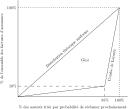
\includegraphics[width = \columnwidth]{img/gini}
%  \caption{Coefficient de Gini et Courbe de Lorentz}
%\end{figure}


%Une lecture de la courbe de Lorentz (figure 1) serait \og les 15\% des assurés les plus risqués paient 90\% de l'ensemble des factures d'assurance \fg{}. Ceci correspond bien au principe de mutualisation des risques qui correspond à la base des systèmes d'assurance. Ainsi, plus le coefficient de Gini est élevé, plus la capacité à individualiser les tarifs sera bonne. La normalisation de ce coefficient permet de s'assurer que la valeur prise par la métrique va de 0 (aucune capacité prédictive) à 1 (capacité prédictive parfaite).

\subsection{Statistiques Descriptives}

Les statistiques descriptives sont faites pour vérifier le type de données traitées, la présence de valeurs manquantes, la présence de valeurs aberrantes et les distributions. De plus, on repère les types de variables (continues, catégorielles, ordinales, etc.) pour spécifier le traitement au cas par cas.

L'inférence faite à partir de modalités rares (moins de 5\% en général) n'est pas robuste et peut conduire à du sur-apprentissage. Les statistiques descriptives sur les variables catégorielles permettent de détecter ces modalités.

Enfin, l'étude des variables continues permet de prévoir l'utilité de transformations (normalisation ou standardisation).

\subsection{Benchmark d'ouverture}

Il est intéressant de placer un benchmark afin d'avoir une valeur de la métrique objectif (Coefficient Normalisé de Gini) à dépasser. Le score obtenu par un Light GBM\footnote{Gradient Boosting Machine} est généralement élevé et rapidement obtenu. Celui-ci est de : 0.2719 par validation croisée sur 5 blocs (5fCV). Bien que le score obtenu est sujet à fluctuer, il est intéressant de refaire un Light GBM après chaque étape de traitement pour voir si les modifications apportées augmente ou diminue le score.


\subsection{Pré-traitement des données}

Le pré-traitement des données consiste essentiellement à la gestion des valeurs manquantes. Plusieurs variables ont été identifiées dans les statistiques descriptives (figure 2). Selon le taux de valeurs absentes, la manipulation appliquée sera différente. 

\begin{figure}[H] \centering
  \includegraphics[width = \columnwidth]{img/missing_values}
  \caption{Valeurs manquantes par variable}
\end{figure}


Deux colonnes présentent trop de valeurs manquantes (plus de 40\%) pour une imputation sophistiquée, ainsi, elles sont remplacées par une valeur spéciale (-999 par exemple) pour conserver l'information issue de l'absence de valeur. En effet, en croisant ces variables avec la cible, il est noté que le taux croisé d'effectif est significativement différent à ceux des valeurs normales.

Pour le reste des variables, une imputation par forêt aléatoire est faite. Le procédé d'imputation est le suivant :
\begin{itemize}
    \item Utiliser uniquement l'échantillon d'apprentissage pour construire la forêt aléatoire.
    \item Modéliser la variable étudiée en s'assurant qu'il s'agisse du bon type d'arbres (classification ou régression) en utilisant les autres variables comme régresseurs.
    \item Prédire les valeurs de la variable étudiée pour l'ensemble des observations manquantes des deux échantillons (apprentissage et test).
    \item Remplacer les valeurs manquantes et s'assurer qu'il n'y a plus de valeurs manquantes pour la colonne traitée.
\end{itemize}

Suite aux imputations faites, le Light GBM de référence renvoie un Gini de 0.2721, toujours par validation croisée sur 5 folds. On note une augmentation par rapport au benchmark bien que la différence soit trop faible pour en tirer des conclusions.

\subsection{Sélection des variables}

Le Light GBM effectué après les imputations permet également d'identifier l'importance des variables dans le pouvoir prédictif du modèle. L'importance d'une variable peut être mesurée de différentes manières. Celle adoptée ici est le \og Gain \fg{}, i.e. la contribution de la variable au modèle. Ainsi, plus une variable contribue au pouvoir prédictif d'un modèle, plus son \og Gain \fg{} associé sera élevé. Arbitrairement, on garde la première moitié des variables les plus contributives au modèle.

\begin{figure}[H] \centering
  \includegraphics[width = \columnwidth]{img/var_imp_lgb}
  \caption{Importance des variables}
\end{figure}


En plus des importances issues du Light GBM, une forêt aléatoire (non paramétrée de façon optimale) est construite pour réaliser une seconde liste d'importance en termes de \og permutation \fg{} (notion équivalente au \og Gain \fg{}). De même, cette seconde liste est issue de la première moitié des variables les plus importantes au modèle. L'union de ces deux listes constitue la liste finale des variables retenues pour la suite. Au total, ce sont 35 régresseurs sur les 57 initiaux qui sont retenus.


\subsection{Traitement des données}

Lors de la phase des statistiques descriptives, plusieurs variables présentaient des modalités rares (effectif inférieur à 5\%). Celles-ci doivent être fusionnées pour pouvoir inférer des résultats robustes (AFDM ou tableaux de contingence).

La stratégie de fusion peut passer par une projection des modalités d'une variable sur le premier plan factoriel d'une AFDM. Chaque modalité rare sera alors associée à la modalité fréquente la plus proche d'elle (et si possible projetée dans la même direction), ou un ensemble de modalités rares peuvent se regrouper pour former un groupe supplémentaire (clusters).

La stratégie de fusion peut également passer par des tableaux de contingence (figure 4) qui croisent les variables problématiques avec la cible. Les modalités rares sont fusionnées soit entre elles si elles se comportent de façon similaire, soit avec une modalité fréquente si le comportement s'y rapproche.

\begin{figure}[H] \centering
  \includegraphics[width = \columnwidth]{img/ex_tabc}
  \caption{Exemple de projection de modalités par croisement}
\end{figure}

\[ * \ * \ * \]

Une variable présente un grand nombre de modalités (104). Plutôt que de fusionner ces modalités, on peut s'en servir comme régresseur unique d'une régression logistique avec la variable cible comme variable à expliquer. Les modalités seront alors remplacées par les coefficients estimés et la variable deviendra alors numérique et continue.

Le Light GBM fournit un score de 0.2729 (5fCV) pour la stratégie par AFDM et de 0.2757 (5fCV) pour la stratégie par tableaux croisés. Le score ayant fortement augmenté pour la seconde stratégie, elle sera retenue pour la suite.

\subsubsection{Normalisation des données}

Certaines variables continues ont une distribution qui se rapprochent d'une distribution normale. Il serait intéressant de tenter de les normaliser à travers différentes méthodes (box-cox, logarithme, racine carré).

\begin{figure}[H] \centering
  \includegraphics[width = \columnwidth]{img/ex_normalisation}
  \caption{Exemple de transformation}
\end{figure}

Il est notable que la transformation de box-cox est la meilleure pour normaliser cette distribution. Cette étude est menée pour les variables continues.

En réutilisant un Light GBM pour mesurer les conséquences des normalisations faites, il est noté que la métrique diminue, suite à chacune des deux stratégies de fusion de modalités. On passe respectivement à un Gini de 0.2729 (AFDM) et 0.2752 (tableaux croisés). Ces diminutions sont minimes mais la normalisation des variables n'est pas obligatoire. Par conséquent, cette étape est laissée de côté pour la suite. 

À la fin de cette étape, le traitement se résume à la fusion de modalités en utilisant des tableaux de contingence.

\subsection{Étude des corrélations et dépendances}

L'objectif de cette étape est de diminuer à nouveau le nombre de variables explicatives. La stratégie est différente : il s'agit d'étudier les corrélations et les dépendances entre variables puis avec la cible. Ceci permet de détecter des problèmes de colinéarité et ou dépendance entre prédicteurs :

\begin{itemize}
    \item les liens entre variables continues se font grâce aux corrélations,
    \item les liens entre les variables continues et la cible se font grâce à un test d'ANOVA,
    \item les liens entre variables catégorielles (et la cible) se font grâce aux V de Cramer\footnote{Le V de Cramer est la statistique du $\chi^2$ standardisée de façon à ce qu'elle varie entre 0 et 1}.
\end{itemize}

Les variables qui dépassent les seuils arbitrairement fixés ou qui ne passent pas le test d'ANOVA sont laissées de côté. Le nombre de prédicteurs chute alors à 29. % TODO

\subsection{Paramétrisation des modèles}

Une dizaine d'algorithmes sont testés pour tenter d'avoir le meilleur pouvoir prédictif. On y trouve des modèles de base (LDA, KNN, régression logistique (pénalisée), SVM), puis des modèles de bagging (RF) et de boosting (ADABoost, GBM, XGBM, LGBM).

L'ensemble des modèles ensemblistes et la régression logistique pénalisée sont optimisés selon leurs paramètres de pré-apprentissage\footnote{Les algorithmes KNN et SVM ne sont pas optimisés faute du temps d'exécution nécessaire au calcul de matrices immenses de distance}.

Pour chaque modèle, la question du ré-échantillonnage est traitée. Pour l'ensemble des modèles, les stratégies de down-sampling, up-sampling et SMOTE sont testées en plus du cas sans sampling.





\section{Méthodes utilisées}
Les deux méthodes à traiter a minima pour notre groupe dans le cadre de ce projet de classification sont la régression logistique pénalisée et le XGboost dont les principes sont radicalement différents.


\subsection{Régression pénalisée}
La pénalisation de la métrique évaluant la prédiction est un principe applicable à toutes les méthodes d'estimation où l’on a des combinaisons linéaires de variables avec des coefficients à estimer (réseaux de neurones, SVM linéaire, etc).\\
L'idée étant que les hypothèses classiques de la régression linéaire permettent d'obtenir le meilleur estimateur non biaisé i.e. l'estimateur sans biais de variance minimale.\\
Dans les faits on obtient un estimateur de faible biais mais de variance plus élevée.\\
Or en considérant l'écart quadratique moyen (EQM) qui est la fonction de perte la plus largement utilisée on a : \[\ E\left[\left(y^{*}-\hat{y}^{*}\right)^{2}\right]=\sigma^{2}+\left(E\left[\hat{y}^{*}\right]-y^{*}\right)^{2}+E\left[\left(\hat{y}^{*}-E\left[\hat{y}^{*}\right]\right)^{2}\right] \]\ 
On a respectivement $\sigma^{2}$ la variance incompressible de la cible Y, le biais et la variable de la prévision. Ainsi si on s'autorise un certain biais, on peut imaginer qu'il est possible de réduire plus que proportionnellement la variance et ainsi gagner en pouvoir prédictif. Pour illustrer ceci, en utilisant les notations de l'équipe scikit-learn on note alors ce problème : 

$\min _{\beta_{1}, \cdots, \beta_{p}} \sum_{i=1}^{n}\left(y_{i}-\sum_{j=1}^{p} \beta_{j} z_{i j}\right)^{2}+\lambda \ R(  \beta) \\ $\text{sous contraintes : }$ R(\beta)\leq \tau$ \\

où l'on aura pris soin de centrer et réduire nos variables afin de leur accorder la même importance.
\\

Il y a donc 3 types de pénalisation utilisés régulièrement: 
\begin{enumerate}
    \item en norme $L^{2}$ on parle alors de régression ridge  : \ $R(\beta)=\sum_{j=1}^{p}\beta_{j}^{2}$
    \item en norme $L^{1}$ on parle alors de régression LASSO  : $R(\beta)=\sum_{j=1}^{p}\left|\beta_{j}\right|$
    \item ElasticNet qui est une combinaison linéaire des 2 : $R(\beta)=\alpha \sum_{j=1}^{p}\left|\beta_{j}\right|+(1-\alpha) \sum_{j=1}^{p} \beta_{j}^{2}$
\end{enumerate}

Notons que $\lambda$ est un paramètre du modèle qu'il faut calibrer également.\\
On a une relation inverse entre $\tau$ et $\lambda$. Lorsque $\lambda=0$ on retrouve les MCO et plus $\lambda$ est grand, plus les coefficients sont contraints (plus de biais, moins de variance).
On peut voir les coefficients se déformer en fonction de $\lambda$.\\
La régression ridge est plus souple que la régression LASSO qui fait converger beaucoup plus vite les coefficients vers 0 ce qui fait qu'on s'en sert comme méthode de sélection de variable.\\Néanmoins, on obtient au maximum N  variables prédictives (identifiabililité) ce qui peut être préjudiciable quand le nombre de variables est très supérieur au nombre d'observations ($p \gg N$).\\
De plus, elle choisit arbitrairement une variable parmi un groupe de variables corrélées quand la regression ridge permet de pondérer les influences.\\
L'Elastic Net permet de combiner les avantages des deux méthodes en contrepartie d'une complexité accrue.\\

Pour déterminer $\lambda$ on procède généralement par apprentissage-test lorsque c'est possible ou par validation croisée K-folds lorsque la base est faible, en minimisant le RMSE. Des formules basées sur des hypothèses simplificatrices existent également.\\
En régression ridge, une astuce permet d'accélérer drastiquement les calculs en validation croisée Leave-One-Out grâce à une décomposition en valeurs singulières de X.\\
Par ailleurs, de manière assez naturelle on obtient l'estimateur avec  $\hat{\beta}_{\text {Ridge}}=\left(X^{\prime} X+\lambda I_{p}\right)^{-1} X^{\prime} y$\\


Pour la régression LASSO, on n'a pas de formulation explicite de $\beta$ (car la fonction valeur absolue n'est pas différentiable) ainsi on procède de manière itérative (LARS, Forward Stagewise). On fait varier de manière sélective les coefficients des variables. En grande dimension, on privilégiera la descente de gradient ou ses variantes pour l'estimation de $\beta$.\\
\subsubsection{Régression logistique pénalisée}
Dans le cadre classique de la discrimination binaire par la régression logistique, on suppose $(x_i,yi)$ IID d'une même distribution inconnue.\\
On modélise $P(Y=1|X=x_i)=\frac{1}{1+e^{-\left(\beta^{\prime} x\right)}}=p_i$.\\
Pour le cas particulier de la régression logistique pénalisée on cherche à minimiser:
\[\ -\frac{1}{n} \sum_{i=1}^{n} \left[y_{i} \ln p_{i}+\left(1-y_{i}\right) \ln \left(1-p_{i}\right)\right] +\lambda \times R(\beta) \]\
Les principes de la pénalisation sont les mêmes que précédemment, seulement on ne pénalise pas la constante mais elle doit faire partie de l'estimation.\\


\subsubsection{Résultats}

\subsection{XGboost}
L’algorithme XGboost est l'abréviation de e\textbf{X}treme \textbf{G}radient \textbf{Boost}ing approche introduite par Friedman.\\
Comme la plupart des méthodes basées sur des arbres de décisions, il peut être utilisé en classication comme en régression.\\
L'approche combine 2 mécanismes : le boosting et la descente de gradient.\\
Le Boosting est une méthode ensembliste qui consiste à agréger des classifieurs élaborés séquentiellement sur un échantillon d’apprentissage dont les poids des individus sont corrigés au fur et à mesure, les individus mal classés se voyant affecter un poids plus important. Les classifieurs sont pondérés selon leurs performances.\\
D'autre part, la descente du gradient est une technique itérative qui permet d’approcher la solution d’un problème d’optimisation.\\
En apprentissage supervisé, la construction du modèle revient souvent à déterminer les paramètres (du modèle) qui permettent d’optimiser une fonction objectif.\\
Enfin, outre les deux mécanismes précédents, l’approche possède aussi des paramètres liés à l’utilisation d’arbres comme classifieurs.\\
Ainsi, l’algorithme XGboost dépend d’un grand nombre de paramètres: 
\begin{enumerate}
    \item Caractéristiques des
arbres individuels : Profondeur T, effectifs minimums de coupe 
\item Constante
d'apprentissage $\eta$
\item Nombre d'arbres K
\item Taux d'échantillonnage des individus $\beta$
\item Échantillonnage des variables
\end{enumerate}
La prévision se base sur K arbres. On construit donc itérativement ces K arbres, à chaque étape on ajoute celui qui minimise une fonction objectif régularisée qui est la somme d'une fonction de perte et d'une fonction de régularisation.\\
\[\ \mathcal{L}=\sum_{i} l\left(\hat{y}_{i}, y_{i}\right)+\sum_{k} \Omega\left(f_{k}\right) \]\
La fonction de perte est généralement la déviance binomiale en classification binaire :\\
 \[\ -\frac{1}{n} \sum_{i=1}^{n} \left[y_{i} \ln p_{i}+\left(1-y_{i}\right) \ln \left(1-p_{i}\right)\right] \]\
On utilise la descente de gradient pour optimiser cet objectif à chaque étape.\\
On peut ajouter de l'aléa dans l'échantillon test en utilisant seulement un échantillonnage des données pour construire les arbres.\\
Ce qui a l'avantage d'accélérer les calculs et de se prémunir contre le surapprentissage.\\
L'algorithme propose également une gestion efficace des valeurs manquantes.\\
On optimise les paramètres de l'algorithme par grid search.\\
Il est évident que plus le nombre d'itérations est grand, plus on s'approche de la solution optimale, cependant celà s'effectue au détriment du temps de calcul.\\
Le compromis pour $\eta$ $\in$ $]0,1[ $ est réalisé entre vitesse de convergence et surapprentissage.\\
Si l'algorithme est très efficace, souple avec le choix des fonctions de coûts,
adaptables à différents problèmes, permettant de prendre efficacement en compte des interactions non linéaires cela reste un modèle difficilement interprétable (même si on peut calculer des mesures d'importance des variables), lourd en mémoire et intensif avec beaucoup de paramètres à optimiser et un risque de surapprentissage qui peuvent rendre sa mise en œuvre efficiente moins aisée.


\subsubsection{Résultats}









\section{Résultats}

\begin{figure}[H] \centering
  \includegraphics[width = \columnwidth]{img/results}
  \caption{Performance de validation des modèles}
\end{figure}

% références
\nocite{*}
\bibliographystyle{acm}
\bibliography{biblio}

\end{multicols}

\end{document}

